\section{Bayesian Analysis}
\label{sec:bayesian}
\emph{In short: the same likelihood with uniform priors, sampled with MCMC: $\Araw=-0.0443$ ($68\%$ interval $[-0.0528,-0.0358]$) with converged chains; the Bayes factor of $A=0$, $BF_{10}\approx9\times10^3$, depends on the prior width.}
The Bayesian analysis takes the likelihood of Sec.~\ref{sec:model} as it is and adds only a prior and a sampler; it changes the question asked of the data, not the model.
\subsection{Priors and Posterior}
\label{sec:bayes_prior}
Bayes' theorem combines the likelihood of Eq.~\eqref{eq:likelihood} (Sec.~\ref{sec:model}) with a prior $\pi(\theta)$ into the posterior
\begin{equation}
p(\theta\mid D)=\frac{\mathcal{L}(D\mid\theta)\,\pi(\theta)}{p(D)},
\label{eq:bayes}
\end{equation}
The priors are uniform, with independent ranges except for the ordering of the background slopes: $N_s,N_b\in(0,5N)$ with $N=19{,}731$, $A,A_b\in(-1,1)$, $\mu\in(5260,5310)\,\MeV$, $\sigma\in(3,40)\,\MeV$, $\lambda_1^{\pm}\in(10^{-5},0.1)\,\MeV^{-1}$, $\lambda_2^{\pm}\in(10^{-5},\lambda_1^{\pm})$, $f_{\pm}\in(0,1)$. The prior density is therefore a constant on the allowed region $\Theta$,
\begin{equation}
\pi(\theta)\propto\mathbf{1}\left[\theta\in\Theta\right],
\label{eq:prior}
\end{equation}
and inside it the posterior is proportional to the likelihood. A flat prior is not invariant under reparametrization, but with $\sim$$2\times10^4$ events the posterior is dominated by the likelihood, as a prior-sensitivity check confirms for $A$. The evidence $p(D)$ is a constant: the MCMC samples $\mathcal{L}\,\pi$ without it, and the Savage-Dickey ratio of Sec.~\ref{sec:bayes_factor} avoids it as well; the marginal posterior of $A$ is the histogram of the $A$ component of the chain.
\subsection{MCMC Sampling and Convergence Diagnostics}
\label{sec:bayes_mcmc}
The posterior was sampled with the affine-invariant ensemble sampler of Goodman and Weare~\cite{goodman_weare} as implemented in \texttt{emcee}~\cite{emcee}: 32 walkers started around the maximum of the posterior, $25{,}000$ steps with the first $1/6$ discarded as burn-in ($6.7\times10^5$ samples, acceptance $0.38$). The integrated autocorrelation time is $\tau\in[147,183]$ steps, so the chain is $N/\tau\geq113$ autocorrelation times long for every parameter, above the threshold of $50$~\cite{emcee} ($\gtrsim3600$ effectively independent samples). Two runs started uniformly over the whole prior box converge to the same single mode. The profile likelihood is tabulated so that the result can be combined with others.
\subsection{Posterior Results and Credible Intervals}
\label{sec:bayes_posterior}

The nominal model with the posterior medians coincides with the fit of Fig.~\ref{fig:freq_jointfit}, which it follows over two orders of magnitude. The marginal posterior on the raw asymmetry gives (median and equal-tailed credible intervals, CI)
\begin{gather*}
\Araw = -0.0443, \\
68\%~\text{CI}~[-0.0528,-0.0358], \\ 95\%~\text{CI}~[-0.0608,-0.0276].
\end{gather*}
The posterior is very close to Gaussian (standard deviation $0.0085$), so equal-tailed and highest-posterior-density intervals coincide; with uniform priors its mode, $-0.0441$, is the maximum-likelihood estimate and the result can be compared directly with the Frequentist fit (Sec.~\ref{sec:frequentist}). The other physics parameters (Fig.~\ref{fig:bayes_corner}) are $N_s=15{,}328\pm133$, $N_b=4404\pm82$, $A_b=-0.040\pm0.018$, $\mu=5284.39\pm0.16\,\MeV$ and $\sigma=18.00\pm0.14\,\MeV$. $A$ is almost uncorrelated with them, which is why profiling (Frequentist) and marginalizing (Bayesian) the nuisance parameters give the same result; the largest correlation, $-0.17$, is with $A_b$: conditioning on $A_b=0$ moves $A$ to $-0.0475$, as the fit with a charge-symmetric background does ($-0.0471$, Sec.~\ref{sec:syst}).

\begin{figure*}[t]
\centering
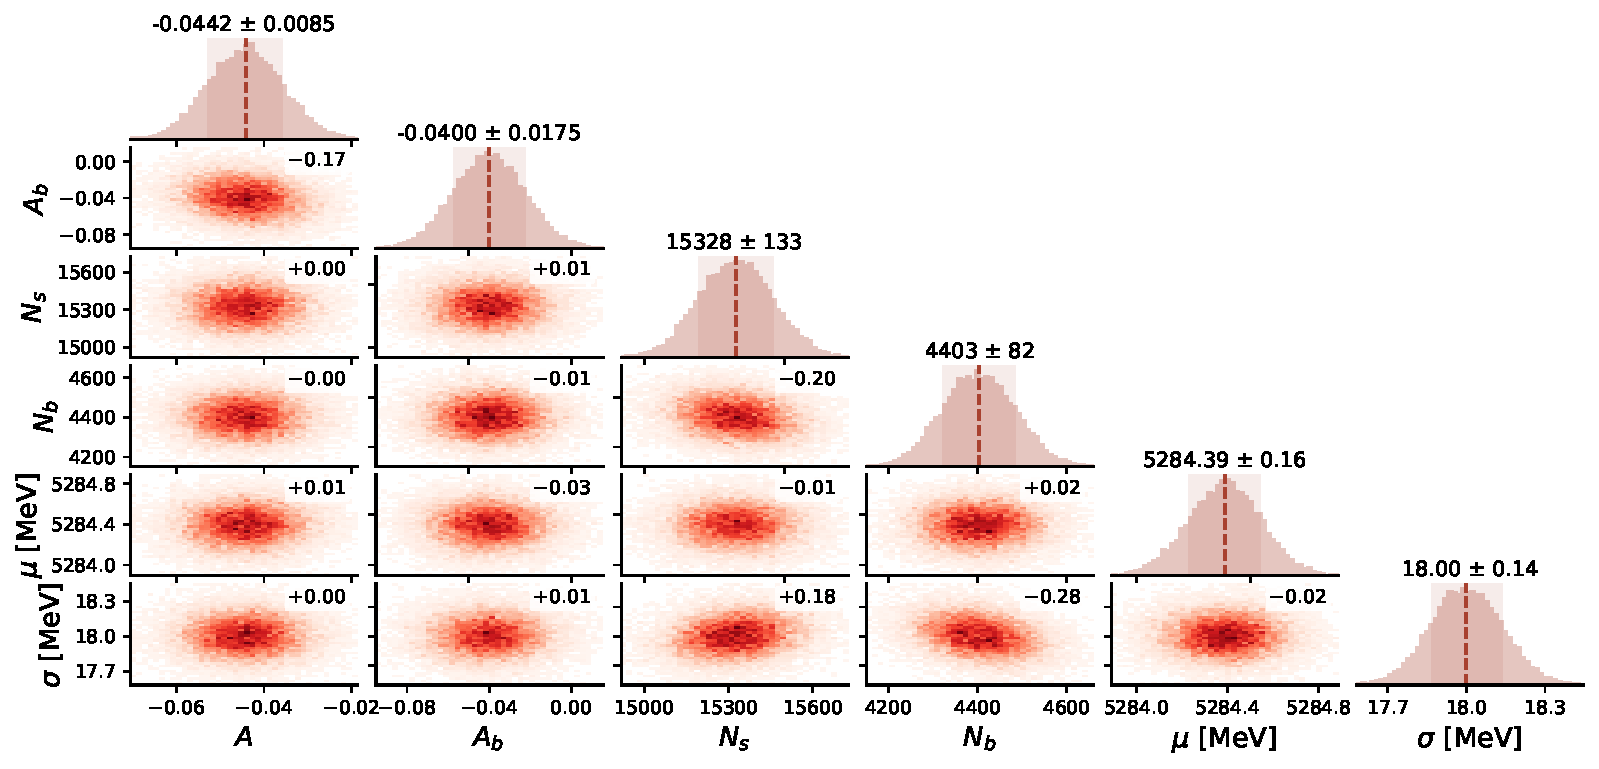
\includegraphics[width=0.78\textwidth]{figures/short_corner.pdf}
\caption{Marginal posteriors and correlations of the six physics parameters of the nominal fit (the six background-shape parameters are marginalized). Diagonal: posterior with its median (line) and $68\%$ interval (band), quoted above as median $\pm$ half-width; below the diagonal: two-dimensional posteriors with the correlation coefficient.}
\label{fig:bayes_corner}
\end{figure*}

\subsection{Bayes Factors}
\label{sec:bayes_factor}
The Bayes factor compares two hypotheses through their evidences, $BF_{10}=P(D\mid H_1)/P(D\mid H_0)$, and requires proper priors. For the nested hypothesis $H_0$: $A=0$ against $H_1$: $A$ free, with shared priors on the other parameters, it reduces to the Savage-Dickey ratio~\cite{dickey1971},
\[
BF_{01} = \frac{p(A=0\mid D)}{\pi(A=0)}, \qquad \pi(A=0)=\tfrac12 .
\]
$A=0$ lies $5.2$ posterior standard deviations from the median, where the chain has essentially no samples, so $p(A=0\mid D)$ was taken from the Gaussian approximation of the marginal posterior: \bnum{BF_{01}\approx1.1\times10^{-4}} ($BF_{10}\approx9\times10^{3}$; Fig.~\ref{fig:bayes_sd}a), \textbf{decisive evidence} against $A=0$ on Jeffreys' scale~\cite{jeffreys}. The value scales with the prior width (Ockham factor): with $A\in(-0.3,0.3)$, $BF_{01}$ drops by a factor $3.3$ and the conclusion is unchanged.

\begin{figure*}[!t]
\centering
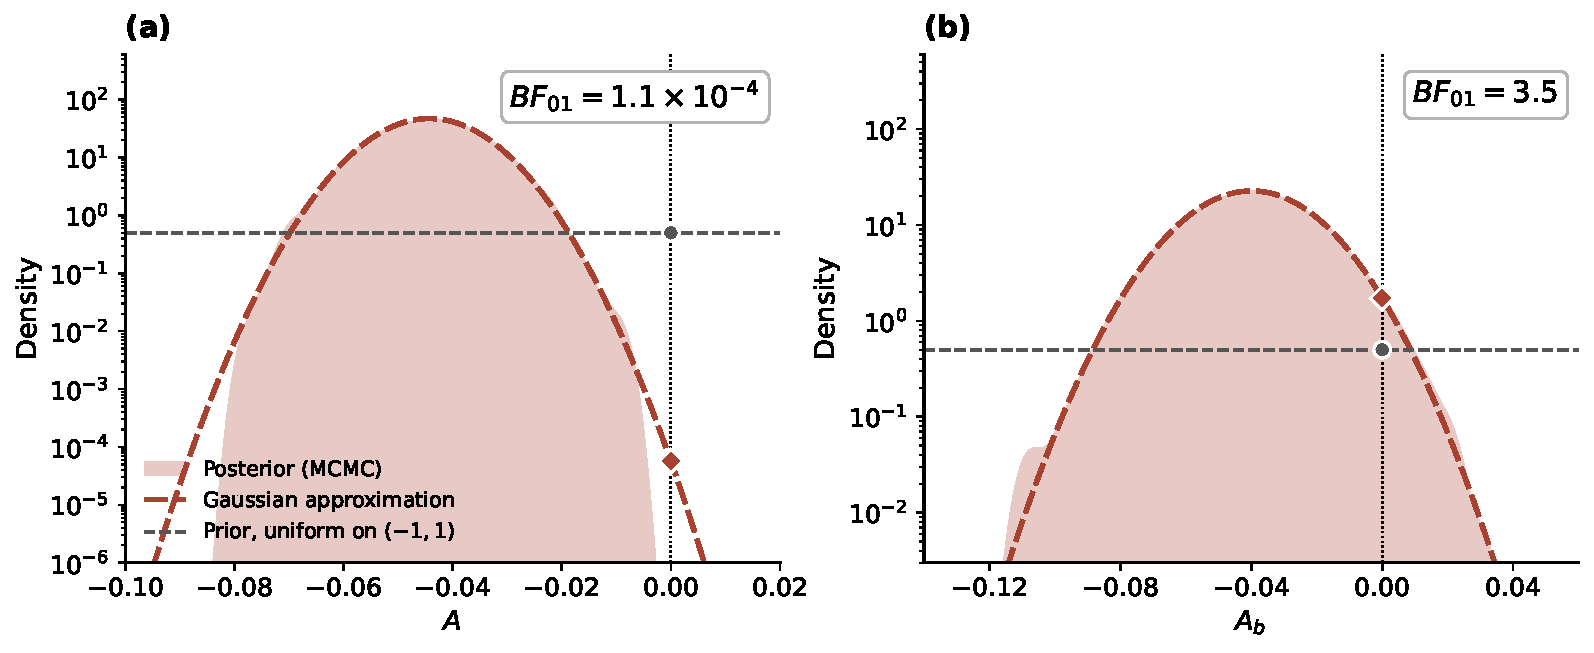
\includegraphics[width=0.78\textwidth]{figures/short_savage_dickey.pdf}
\caption{Savage-Dickey ratio for (a) $A$ and (b) $A_b$: marginal posterior (histogram of the chain and Gaussian approximation) and prior density, logarithmic scale. The Bayes factor $BF_{01}$ is the ratio of the two densities at zero (dots). For $A$ the posterior density at zero is $10^{-4}$ times the prior one; for $A_b$, $2.3$ standard deviations from zero, it is higher than the prior density, and the data favor $A_b=0$.}
\label{fig:bayes_sd}
\end{figure*}

The same test on the background asymmetry shows the Ockham factor at work: $A_b=-0.040\pm0.018$ is $2.3$ standard deviations from zero, yet $BF_{01}(A_b=0)\approx3.5$ (Fig.~\ref{fig:bayes_sd}b), because the likelihood gain does not compensate for spreading the prior; unlike for $A$, the preference changes sign with the prior width. Of the Bayesian results \emph{only the Bayes factor} depends on the prior; the interval of $A$ does not (Sec.~\ref{sec:bayes_posterior}). %A negative $A_b$ is plausible given the misidentified $B^\pm\to K^\pm\pi^+\pi^-$ and $\pi^\pm K^+K^-$ decays;
$A_b$ is kept free in the nominal model and fixing it to zero is one of the systematic variants (Sec.~\ref{sec:syst}).
\subsection{Additional Results}
\emph{Intervals.} Equal-tailed and highest-posterior-density $68\%$ intervals coincide for $A$ and $A_b$ and differ for the skewed parameters; the profile likelihood is tabulated for combination with other results.
\emph{Priors.} No change of the prior on the nuisance parameters or of its parametrization moves $A$ by more than $0.0002$, and the evidence by direct integration agrees in order of magnitude with the Savage-Dickey ratio.
\emph{Model adequacy.} The model does not reach $\chi^2/\mathrm{ndof}\approx1$ ($164.1/88$), because the signal tails are heavier than a Gaussian, but $\Araw$ changes by $-0.0002$ with a Crystal Ball signal; the posterior predictive check reproduces the asymmetry in slices of the mass ($p_B=0.67$, the posterior predictive $p$-value, i.e.\ the fraction of replicas whose discrepancy exceeds the observed one) and puts the difference of the $\chi^2$ of the two charges at the edge of the replicas ($p_B=0.08$).
\emph{Robustness and coverage.} $\Araw$ agrees between the magnet polarities ($0.7\sigma$); $200$ toy-MC experiments give coverage $0.65\pm0.03$ ($68\%$) and $0.93\pm0.02$ ($95\%$) with pulls of width $1.04$.
